\subsection{Physical validation}
We also have tested the planner and controller on the open source hardware platform of F1Tenth vehicle.
This is to show the practicality of our simple reactive planning and control in the presence of noise, unstructured environment, and limited computational resource.
For example, Hokuyo UST-10LX LiDAR provides a new point-cloud every 25 milliseconds, but our planning and control is an order of magnitude faster on the Nvidia Jetson TX2's CPU so we can process every point-cloud.

We tested the car in two tracks.
The simpler one is shown in Fig.~\ref{fig:physical_track} where the track boundaries is mostly structured using corrugated cardboard rolls.
%
The harder track (provided in the videos) is an office with chairs and tables around the office walls and in the middle of the office.
%
Our algorithm manages to successfully complete a lap while avoiding obstacles on both these tracks.

\begin{figure}[!t]
\centering
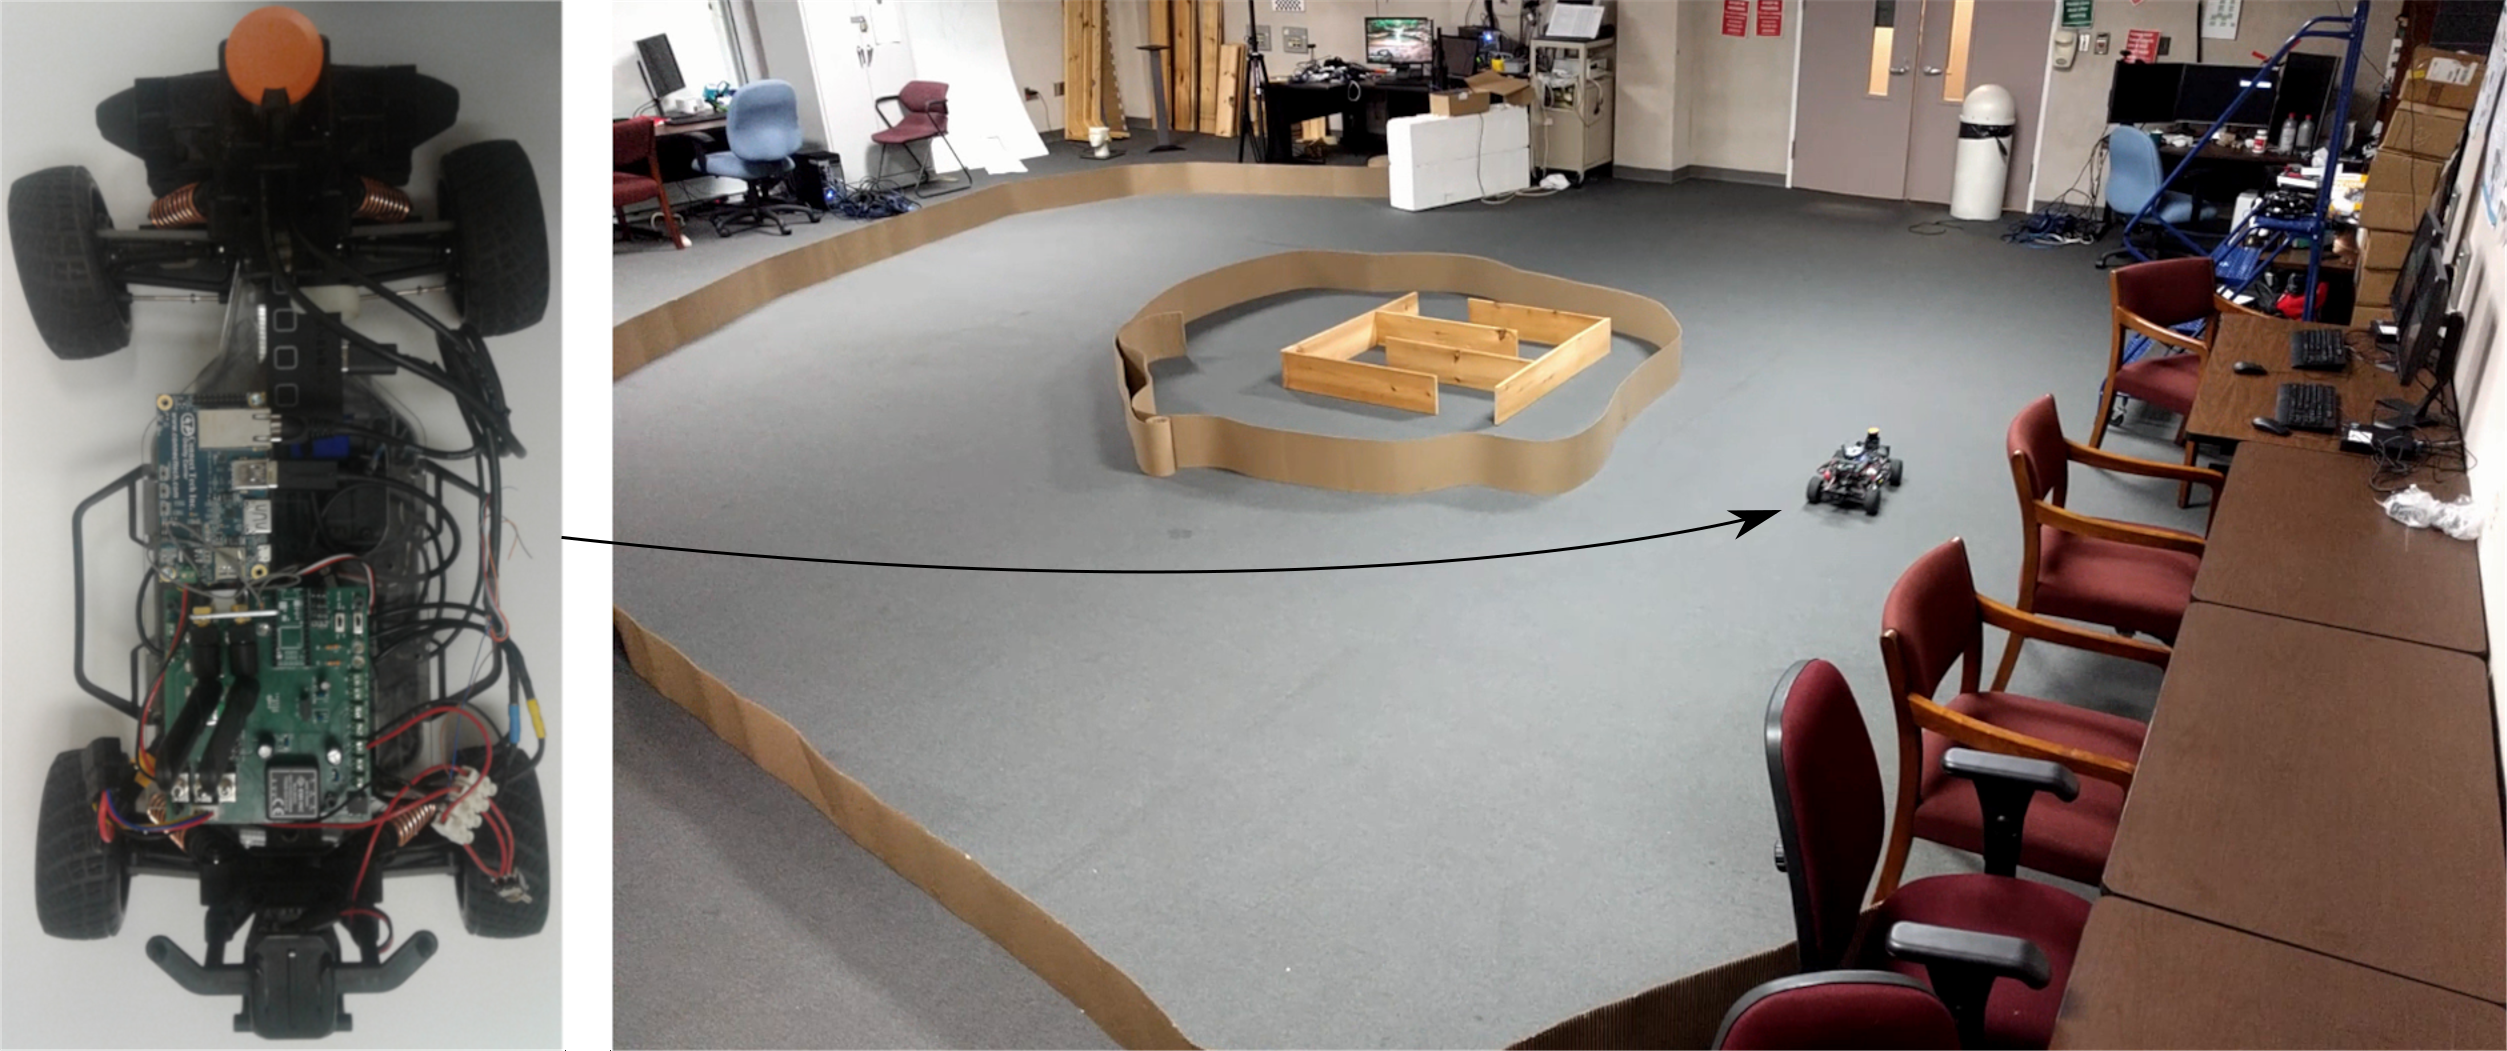
\includegraphics[width=85mm]{Figures/physical_track.png}
\caption{Physical validations.}
\label{fig:physical_track}
\end{figure}


% Our vehicle layout (for the F1/10 competition) is shown in Fig.~\ref{fig:carlayout}.
% The main hardware components are listed below.  
% \begin{itemize}
%     \item Traxxas 1/10 Scale AWD Ford Fiesta ST Rally Race Car
%     \item Velineon 3500 brushless DC motor
%     \item Enertion FOCBOX VESC Speed Controller HW V1.7
%     \item Hokuyo UST-10LX LiDAR
%     \item Nvidia Jetson TX2
%     \item Orbitty carrier board (for TX2)
% \end{itemize}

% \begin{figure}[!t]
% \centering
% 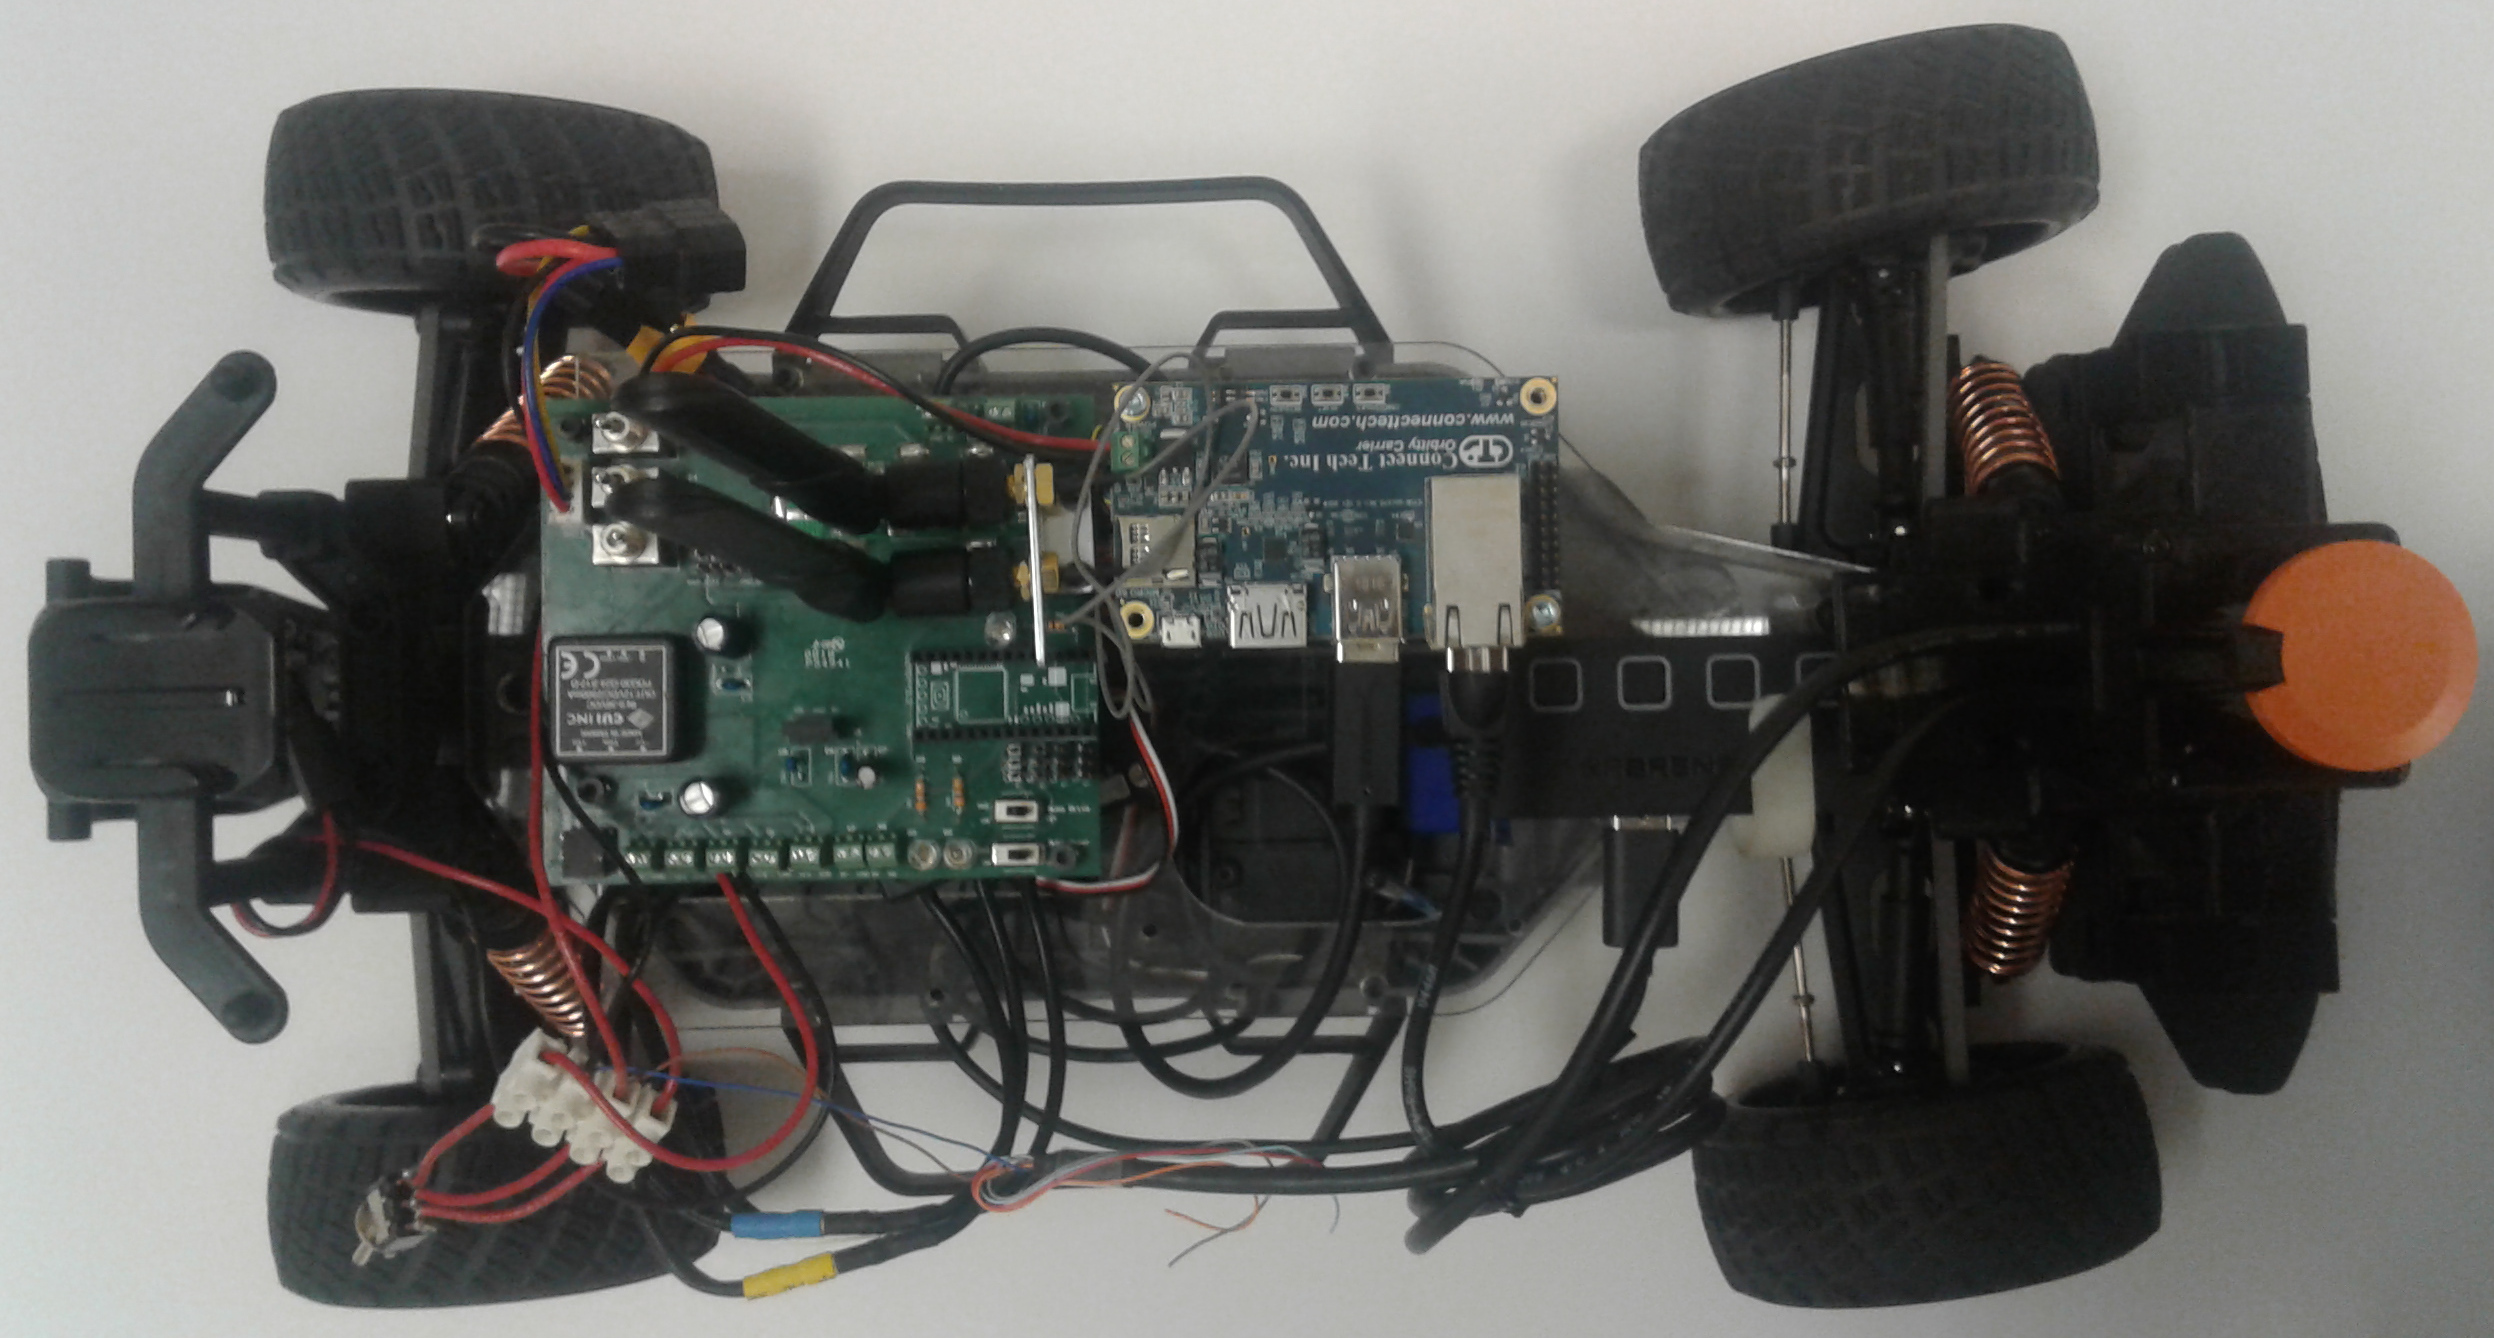
\includegraphics[width=\columnwidth]{Figures/car_f1tenth.jpg}
% \caption{Vehicle Layout}
% \label{fig:carlayout}
% \end{figure}

